This section describes the representations underpinning our approach. First we describe the kernel density representation  that underpins all the models. The representation of the surface features necessary to encode the contact models follows. Finally we describe the form of the contact model and the hand configuration model. In the rest of the paper we assume that the robot's hand is formed of $N_L$ rigid \emph{links}: a palm, and a number of finger phalanges or links. We denote the set of links $L =\{L_i\}$. The representations are summarised at a high level in a video attached as Extension 2.


%Our approach then relies on a pair of models that capture two complementary aspects of the grasping process using this hand representation. The first, referred to as the \emph{contact model}, captures the 3D pose of one hand link $\rl$ \emph{relative} to local features from the object's surface. Given the 3D model of an object that the robot has not grasped yet, contact model $\cm$ allows the robot to compute a set of poses for the corresponding robot link $\rl$. The second model, referred to as the \emph{hand configuration model}, models a set of hand shapes that are compatible with the grasp. The role of the hand configuration model during grasp generation is to constrain the search space. Both models are learned from the same grasp data.

%The remainder of this section details the parametrisation of object surfaces, the contact model, and the hand configuration model.

\subsection{Kernel Density Estimation}



\label{sec:kde}

Much of our work relies on the probabilistic modelling of surface \emph{features}, extracted from 3D object scans. Features are composed of a 3D position, a 3D orientation, and a 2D local surface descriptor that encodes local curvatures. The next section explains in detail the physical observations modelled by those features. In this section, we define the mathematical tools that enable the models discussed below.

Let us denote by $SO(3)$ the group of rotations in three dimensions. A feature belongs to the space $SE(3) \times \mathbb R^2$, where $SE(3) = \mathbb R^3 \times SO(3)$ is the group of 3D \emph{poses} (a 3D position and 3D orientation), and surface descriptors are composed of two real numbers. This paper makes extensive use of probability density functions (PDFs) defined on $SE(3) \times \mathbb R^2$. This section explains how we define these density functions. We represent PDFs non-parametrically with a set of $K$ features (or particles) $x_j$
\begin{equation}
S = \left\lbrace x_j : x_j \in \mathbb R^3 \times SO(3) \times \mathbb R^2 \right\rbrace_{j \in [1,K]}.
\end{equation}
The probability density in a region of space is determined by the local density of the particles in that region. The underlying PDF is created through \emph{kernel density estimation} \cite{silverman1986a}, by assigning a kernel function $\mathcal{K}$ to each particle supporting the density, as
\begin{equation}\label{eq:d}
\pdf(x) \simeq \sum_{j=1}^K w_j \mathcal{K}(x| x_{j}, \sigma),
\end{equation}
where  $\sigma \in \mathbb R^3$ is the kernel bandwidth and $w_j \in \mathbb R^{+}$ is a weight associated to $x_j$ such that $\sum_j w_j = 1$. We use a kernel that factorises into three functions defined on the three components of our domain, namely $\mathbb R^3$, $SO(3)$, and $\mathbb R^2$. Let us denote the separation of feature $x$ into $p \in \mathbb R^3$ for position, a quaternion $q \in SO(3)$ for orientation, $r \in \mathbb R^2$ for the surface descriptor. Furthermore, let us denote by $\mu$ another feature, and its separation into position, orientation and surface descriptor. Finally, we denote by $\sigma$ a triplet of real numbers:
\begin{subequations}
\begin{align}
x &= (p, q, r),\\
\mu &= (\mu_p, \mu_q, \mu_r),\\
\sigma &= (\sigma_p, \sigma_q, \sigma_r).
\end{align}
\label{eq:feature}
\end{subequations}
We define our kernel as
\begin{equation}\label{eq:kernel_in_se3}
\mathcal{K}(x| \mu, \sigma) = \mathcal{N}_3(p| \mu_p, \sigma_p) \Theta(q| \mu_q, \sigma_q) \mathcal{N}_2(r| \mu_r, \sigma_r)
\end{equation}
where $\mu$ is the kernel mean point, $\sigma$ is the kernel bandwidth, and where $\mathcal{N}_n$ is an $n$-variate isotropic Gaussian kernel, and ${\Theta}$ corresponds to a pair of antipodal von Mises-Fisher distributions which form a Gaussian-like distribution on $SO(3)$ (for details see \cite{fisher1953a,sudderth2006a}). The value of ${\Theta}$ is given by
\begin{equation}
\Theta(q|\mu_q, \sigma_q) = C_4(\sigma_q) \frac {e^{\sigma_q \; \mu_q^T q} + e^{-\sigma_q \; \mu_q^T q}}2
\end{equation}
where $C_4(\sigma_q)$ is a normalising constant, and $\mu_q^T q$ denotes the quaternion dot product.

We note that thanks to the nonparametric representation used above, conditional and marginal probabilities can easily be computed from \eq\eqref{eq:d}. The marginal density $\pdf(r)$ is computed as
\begin{align}\label{eq:marginal}
\pdf(r) & \\
      = & \iint \sum_{j=1}^K w_j \mathcal{N}_3(p| p_i, \sigma_p) \Theta(q| q_i, \sigma_q) \mathcal{N}_2(r| r_i, \sigma_r) \textnormal{d}p\textnormal{d}q \\
      = &  \sum_{j=1}^K w_j \mathcal{N}_2(r| r_j, \sigma_r),
\end{align}
where $x_j = (p_j, q_j, r_j)$.
The  conditional density $\pdf(p,q|r)$ is given by
\begin{align}\label{eq:conditional}
\pdf(p,q|{r}) & = \frac{\pdf(p, q, {r})}{\pdf({r})} \\
                   & = \frac{\sum_{j=1}^K w_j \mathcal{N}_2({r}| r_j, \sigma_r) \mathcal{N}_3(p| p_j, \sigma_p) \Theta(q|q_j, \sigma_q)}{\sum_{j=1}^K w_j \mathcal{N}_2({r}| r_j, \sigma_r)}. 
\end{align}

\subsection{Surface Features}
\label{sec:surface_features}

This section explains how the surface features discussed above are acquired from real object data. All objects considered in the paper are represented by point clouds constructed from one or multiple shots taken by a depth camera. A depth camera captures a set of points distributed in a 3D space along the object's visible surface. We directly augment these points with a surface normal. As a result, the point clouds discussed below are composed of points that belong to $SE(3)$. We denote position and orientation as $p$, $q$. The surface normal at $p$ is computed from the nearest neighbours of $p$ using a PCA-based method (e.g. \cite{kanatani2005statistical}). 

\subsection{Contact Model}\label{sec:contact.model}

A contact model $\cm_i$ encodes the joint probability distribution of surface features and of the 3D pose of the $i$-th hand link. Let us consider the hand grasping some given object. The (object) contact model of link $\rl_i$ is denoted by
\begin{equation}\label{eq:M}
\cm_i(U, R) \equiv \pdf^\cm_i(U, R)
\end{equation}
where $\cm_i$ is short for $\pdf^\cm_i$, $R$ is the random variable modelling surface features, and $U$ models the pose of $\rl_i$ \emph{relative} to a surface feature. In other words, denoting realisations of $R$ and $U$ by $r$ and $u$, $\cm_i(u, r)$ is proportional to the probability of finding $\rl_i$ at pose $u$ relative to the frame of a nearby object surface feature that exhibits feature vector equal to $r$.

Given a set of surface features $\lbrace x_j \rbrace_{j=1}^{K_O}$, with $x_j = (v_j, r_j)$ and $v_j = (p_j, q_j)$, a contact model $\cm_i$ is constructed from features from the object's surface.  Surface features  close to the link surface are more important than those lying far from the surface. Features are thus weighted, to make their influence on $\cm_i$  decrease with their squared distance to the $i^\textnormal{th}$ link (\fig\ref{fig:representations.modeldist.cont}). Additionally, features that are further than a cut-off distance $\delta_i$ from $\rl_i$ are ignored. We opted for a weighting function whose value decreases exponentially with the square distance to the link:
\begin{equation}
w_{ij} = \begin{cases}\exp(-\lambda ||p_j-a_{ij}||^2) \quad &\textnormal{ if } ||p_j-a_{ij}|| < \delta_i\\
0 \quad &\textnormal{ otherwise},\end{cases}
\label{eq:learning.modeldist.wgh}
\end{equation}
where $\lambda \in \mathbb R^{+}$ and $a_{ij}$ is the point on the surface of $\rl_i$ that is closest to $p_j$. The intuitive motivation for this choice is that we require a weight function that falls off quickly so as to constrain each contact model to a limited volume around the related links. This means that the contact model will only take account of the local shape, while falling off smoothly. A variety of monotonic, fast declining functions could be used instead.

Let us denote by $u_{ij} = (p_{ij}, q_{ij})$ the pose of $\rl_i$ relative to the pose $v_j$ of the $j^{\mathnormal{th}}$ surface feature. In other words, $u_{ij}$ is defined as
\begin{equation}
u_{ij} = v_j^{-1} \circ s_i,
\label{eq:local.pose}
\end{equation}
where $s_i$ denotes the pose of $\rl_i$, $\circ$ denotes the pose composition operator, and $v_j^{-1}$ is the inverse of $v_j$, with $v_j^{-1} = (-q_j^{-1}p_j, q_j^{-1})$ (see \fig\ref{fig:representations.model}). The contact model is estimated as
\begin{equation}
\cm_i(u,r) \simeq \frac 1Z \sum^{K_{M_i}}_{j=1} w_{ij}\mathcal{N}_3(p|{p_{ij}}, \sigma_{p}) \Theta(q|{q_{ij}}, \sigma_{q}) \mathcal{N}_2(r|{r_j}, \sigma_{r})
\label{eq:cm}
\end{equation}
where $Z$ is a normalising constant, $u = (p, q)$, and where $K_{M_i} \leq K_O$ is a number of features which are within cut-off distance $\delta_i$ to the surface of link $\rl_i$. If the number of features $K_{M_i}$ of contact model $\cm_i$ is not sufficiently large, contact model $\cm_i$ is not instantiated and is excluded from any further computation. Consequently, the overall number of contact models $N_M$ is usually smaller than the number of links $N_L$ of the robotic hand. We denote the set of contact models learned from a grasp example $g$ as $\mathcal{M}^g=\{\mathcal{M}^g_i\}$. The contact models are quite different for the different links within a grasp. This can be seen by comparing the marginalised contact models $\cm(r)$ for two example training grasps and two links in \fig\ref{fig:representations.features}.

%Sum~\eqref{eq:cm} involves only terms for which $x_j = ((p_j, q_j), r_j)$ belong to the neighbourhood of $\rf_i$, $\lbrace x_j: ||p_j-a_{ij}|| \leq \delta, \delta \in \mathbb R^{+} \rbrace$. If the neighbourhood of a particular link $i$ is empty, i.e. $K_{M_i} = 0$, the corresponding contact model is not instantiated and it is excluded from any further computation.
\begin{figure}[t]
\centerline{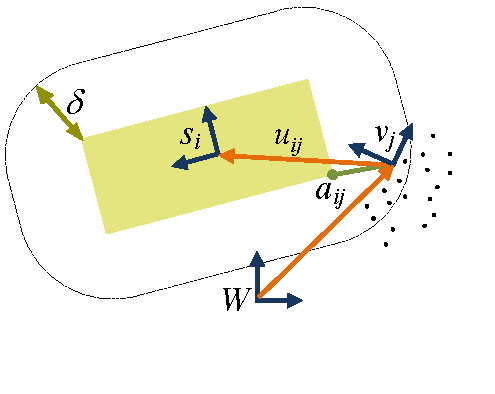
\includegraphics[width=5cm]{resources/model}}
\caption[Contact model]{Contact model. The figure shows the $i$-th link $\rl_i$ (solid block) and its pose $s_i$. The black dots are samples of the surface of an object. The distance $a_{ij}$ between a feature $v_j$ and the closest point on the link's surface is shown. The rounded rectangle illustrates the cut-off distance $\delta_i$. The poses $v_j$ and $s_i$ are expressed in the world frame $W$. The arrow $u_{ij}$ is the pose of $\rl_i$ relative to the frame for the surface feature $v_j$.}
\label{fig:representations.model}
\end{figure}

The parameters $\lambda$ and $\sigma_{p}$, $\sigma_{q}$, $\sigma_{r}$ were chosen empirically and kept fixed in all experiments reported in \sect\ref{sec:method}. The time complexity for learning each contact model from an example grasp is $\Omega(T K_O)$ where $T$ is the number of triangles in the tri-mesh describing the hand links, and $K_O$ is the number of points in the object model.


%\begin{figure}[t]
%\centering{
%\subfloat[]{\includegraphics[height=3.4cm]{resources/example1}}\quad
%\subfloat[]{\includegraphics[height=3.4cm]{resources/example2}}\quad
%\subfloat[]{\includegraphics[height=3.4cm]{resources/example5}}
%}
%\caption[Hand-object contact]{Example top grasp of a mug represented by a point cloud (panel a). The dotted regions are rays between features and the closest hand link surfaces (panel b). The black curves with frames at the fingertips represent the range of hand configurations in \eq\eqref{eq:hc} (panel c).}
%\label{fig:representations.modeldist.cont}
%\end{figure}

\subsection{Hand Configuration Model}

The hand configuration model, denoted by $\hc$, encodes a set of configurations of the hand joints $h_c \in \mathbb R^D$ (i.e., joint angles), that are particular to a grasp example. The purpose of this model is to allow us to restrict the grasp search space (during grasp transfer) to hand configurations that resemble those observed while training the grasp.

In order to boost the generalisation capability of the grasping algorithm the hand configuration model encodes the hand configuration that was observed when grasping the training object, but also a set of configurations recorded during the approach towards the object. Let us denote by $h^t_c$ the joint angles at some small distance \emph{before} the hand reached the training object, and by $h^g_c$ the hand joint angles at the time when the hand made contact with the training object. We consider a set of configurations interpolated between $h^t_c$ and $h^g_c$, and extrapolated beyond $h^g_c$, as
\begin{equation}
h_c(\gamma) = (1 - \gamma)h^g_c + \gamma h^t_c
\label{eq:learning.configmodel.config}
\end{equation}
\noindent where $\gamma \in \mathbb R$. For all $\gamma < 0$, configurations $h_c(\gamma)$ are beyond $h^g_c$ (see \fig\ref{fig:representations.modeldist.cont}). The hand configuration model $\hc$ is constructed by applying kernel density estimation to \begin{equation}\label{eq:H_c}\mathcal H_c = \lbrace h_c(\gamma): \gamma \in [-\beta, \beta], \beta \in \mathbb R^{+}\rbrace,\end{equation} as 
\begin{equation}
\hc(h_c) \equiv \sum_{\gamma \in [-\beta, \beta]} w({h_c(\gamma)}) \mathcal{N}_D(h_c|h_c(\gamma), \sigma_{h_c}) 
\label{eq:hc}
\end{equation}
where  $w({h_c(\gamma)}) = \exp(-\alpha \|h_c(\gamma) - h^g_c \|^2)$ and $\alpha \in \mathbb R^{+}$. $\alpha$ and $\beta$ were hand tuned and kept fixed in all the experiments. The hand configuration model computation has time complexity $\Omega(d_h K_C)$ where $d_h$ is the number of dimensions of the configuration vector, and $K_C$ is the size of the set of values of $\gamma$ used in \eq\eqref{eq:hc}.

\subsection{Reach to Grasp Trajectory}


